
	
	\chapter{Half cycle -hc}
	Suppose that there are two facts $u_i, u_j$ and action with only one effect $<u_i,u_j>$ and no precondition. Then, if there is no other producer of $u_j$, nor any other action that needs $u_i$, $u_i$ is not in init and $u_j$ is not in goal, then whenever when $u_i$ is added, the only possible way to add $u_j$ is to use the action. Therefore we replace $u_j$ by $u_i$, remember that information and use it while expanding plan.
	
	Note that there must not be opposite effect ($<u_j,u_i>$) in any other action \todo{Where is this in specification?}. In such situation -mv can be executed.

	\begin{figure}
		\begin{subfigure}[b]{0.4\textwidth}
			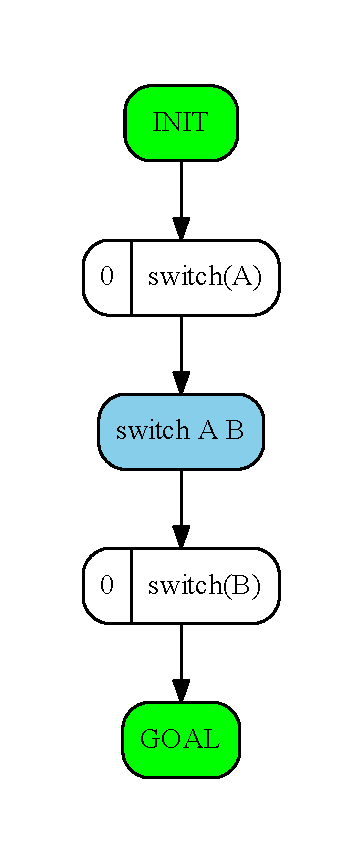
\includegraphics[scale=0.4]{halfCycle/figures/simple_input}
			\caption{before reduction}
		\end{subfigure}	
		\begin{subfigure}[b]{0.4\textwidth}
			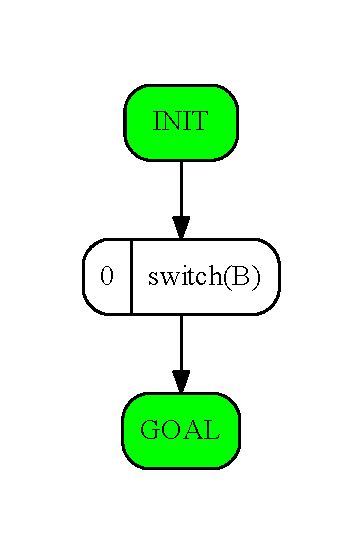
\includegraphics[scale=0.4]{halfCycle/figures/simple_output}
			\caption{after reduction}
		\end{subfigure}
		\caption{Example where facts \emph{0 switched(A)} and \emph{0 switched(B)} can be merged together because there is action \emph{switch A B} meeting all conditions for -hc reduction. }
	\end{figure}


	\section{Reduce operation}
	Let's have SAS in form $<\vars, \init, \goal, \actions, \mutexes{}>$. 
	
	In order to execute this operation there must be values $u_i, u_j$ and action $a$ such that:
	
	\begin{enumerate}
		\item $\var{u_i} = \var{u_j}$
		\item $u_j \notin \init$ \todo{why?}
		\item $u_i \notin \goal$ \todo{why?}
		\item $<u_i,u_j> \in \eff{a}$
		\item $|\eff{a}| = 1$
		\item $|\pre{a}| = 0$
		\item $\con{u_i} = 1$
		\item $\pro{u_j} = 1$ \todo{not necessary}
	\end{enumerate}
	
	The operation does following things:
	
	\begin{enumerate}
		\item replace $u_j$ by $u_i$ in actions and mutexes, and in goal if needs be
		\item remove $u_j$ from $\dom{\var{u_j}}$		
	\end{enumerate}
	
	Output of the reduction is SAS $<\vars{}', \init{}, \goal{}, \actions{}', \mutexes{}'>$.
	
	
	\section{Possible outgoing states of SAS}
	\begin{enumerate}
		\item -mv, -mo, maybe -sd and some other
	\end{enumerate}
	
	\section{States before application of this operation}
	\begin{itemize}
		\item from the beginning
		\item after -mo, -mv, -dv
	\end{itemize}
	
	
	\section{Reverse operation}
	Removed action is added back to SAS. While extending the plan, the plan is traversed and simulated. If $\var{u_i}$ is in state $u_i$ and the next operation needs $u_j$, then $a$ is added to the plan. Extended plan is returned.
	
	\section{Implementation notes}
	Simple implementation without any caching. Possible extension of this operation to search not action that works with 
	
	
	
	
	